\chapter{没入型歩行感覚提示システム}

\thispagestyle{myheadings}

\section{はじめに}
本章では,ベッド型の下肢リハビリを拡張する,下肢リハビリへのモチベーションを向上させるための没入型歩行感覚提示システムについて述べる.提案システムは没入感が高を高めるため,現実的な3DCGを利用し実現する.センサが内蔵されたHMDを使用することで,リハビリ患者の頭部の動きに追従した映像提示により,没入感が高まることが期待できる.次節以降に提案システムの概要,処理の流れについて述べる.

\section{KinectV2を使用したシステム構成}
提案システムでは,ベッド型の下肢リハビリ装置の下肢可動部にKinectV2\cite{KinectV2}を置き,歩行の検出を行う.KinectV2を図\ref{fig:kinect}に示す.KinectV2をセンサとして使用する.提案システムの歩行の検出にKinectV2を使用したシステム構成を図\ref{fig:beforesystemarc}に示す.ベッド型の下肢リハビリ装置の下肢部分の手前にKinectV2を設置する.処理の流れを図\ref{fig:片桐1}に示す.KinectV2からの取得した映像を二値化行い,図\ref{fig:kinectsystemarc}に示す,ベッド型の下肢リハビリ装置の下肢可動部の検出を行う.図\ref{fig:kinectsystemarc}に示す矩形の重心点の座標を取得し閾値を設定し,歩行判定を行う.歩行判定を基にキャラクタは歩行動作を行う.

\begin{figure}[tbp]
	\centering
			\includegraphics[width=0.8\textwidth,angle = 270]{chap2-figure/kinect.eps}
	\caption{KinectV2}
	\label{fig:kinect}
\end{figure}

\begin{figure}[tbp]
	\centering
			\includegraphics[width=0.8\textwidth]{chap2-figure/beforesystem.eps}
	\caption{KinectV2を使用したシステム構成図}
	\label{fig:beforesystemarc}
\end{figure}

\begin{figure}[tbp]
	\centering
			\includegraphics[width=0.3\textwidth]{chap2-figure/katagiri1.eps}
	\caption{処理の流れ}
	\label{fig:片桐1}
\end{figure}

\begin{figure}[tbp]
	\centering
			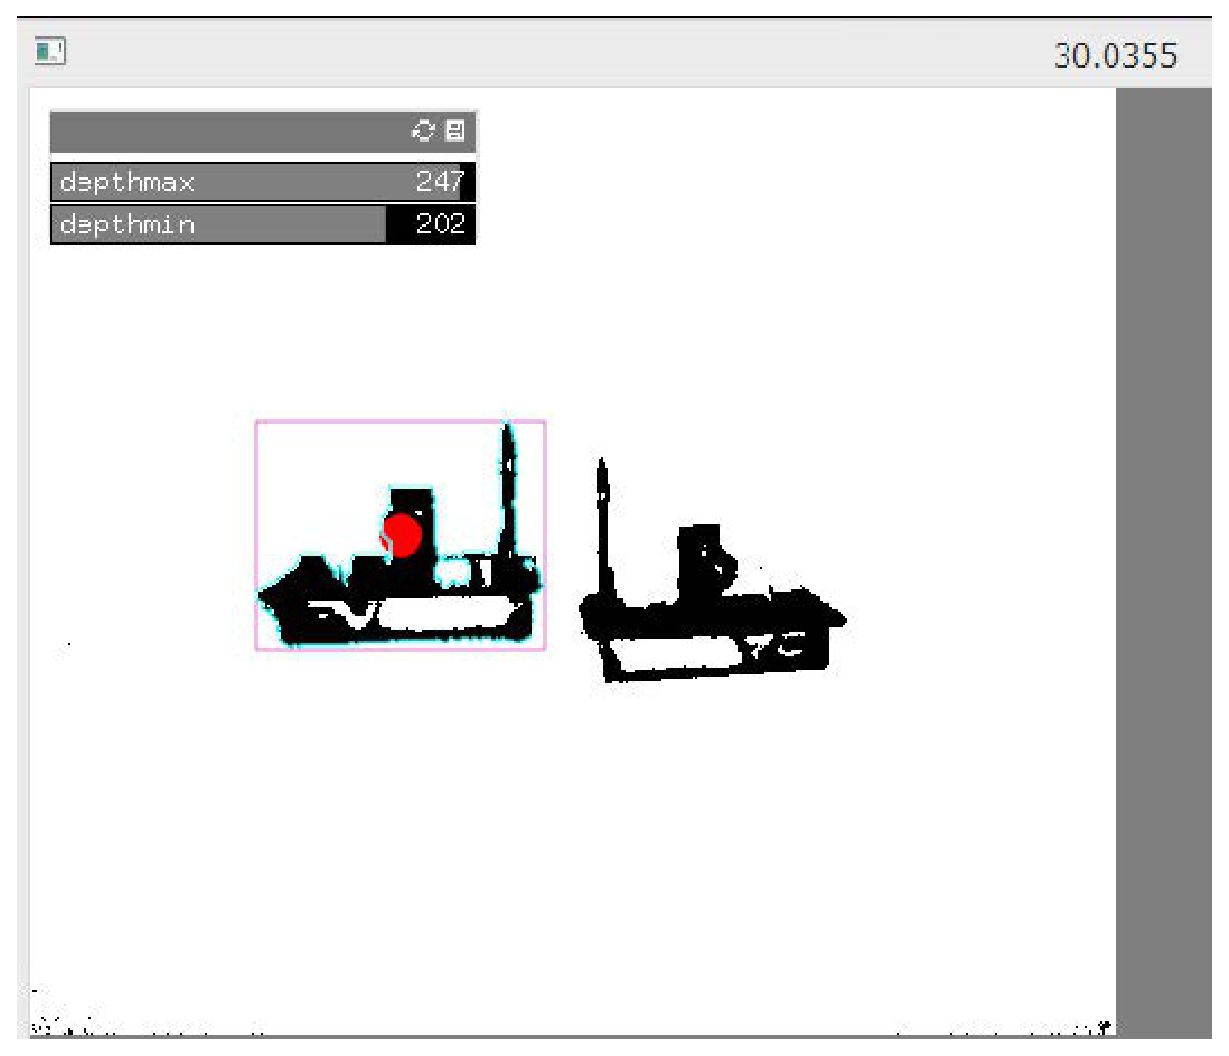
\includegraphics[width=0.8\textwidth]{chap2-figure/kinectsystem.eps}
	\caption{KinectV2の検出画像}
	\label{fig:kinectsystemarc}
\end{figure}


\section{改善を行った没入型歩行感覚提示システムの概要}
KinectV2を使用した提案システムでは,ベッド型リハビリ装置の下肢可動部の検出が困難であったため,提案システムの改善を行う.
改善を行った提案システムは,ベッド型の下肢リハビリ装置に患者は仰向けの体勢をとり,HMDを装着する.提案システムの構成図を図\ref{fig:systemarc}に示す.あらかじめ用意した,仮想空間内をCGキャラクタが歩行動作を行い,CGキャラクタの一人称視点の映像を患者に提示し正常な歩行の想像の助けとする.次節以降にそれぞれの処理について述べる.

\begin{figure}[tbp]
	\centering
			\includegraphics[width=0.8\textwidth]{chap2-figure/system.eps}
	\caption{システム構成図}
	\label{fig:systemarc}
\end{figure}

\section{仮想空間の一例}
仮想空間は3D都市モデル空間を使用している.3D都市モデル空間の例を図\ref{fig:akihabare}--\ref{fig:ue}に示す.3D都市モデル空間は,複数のモデル都市の実際の町並みを基に再現しており,現実的な仮想空間を再現することが可能なモデルである.自作することも可能であるが,臨場感を出すため地図データを用いた3D都市モデルを使用する.

\begin{figure}[tbp]
	\centering
			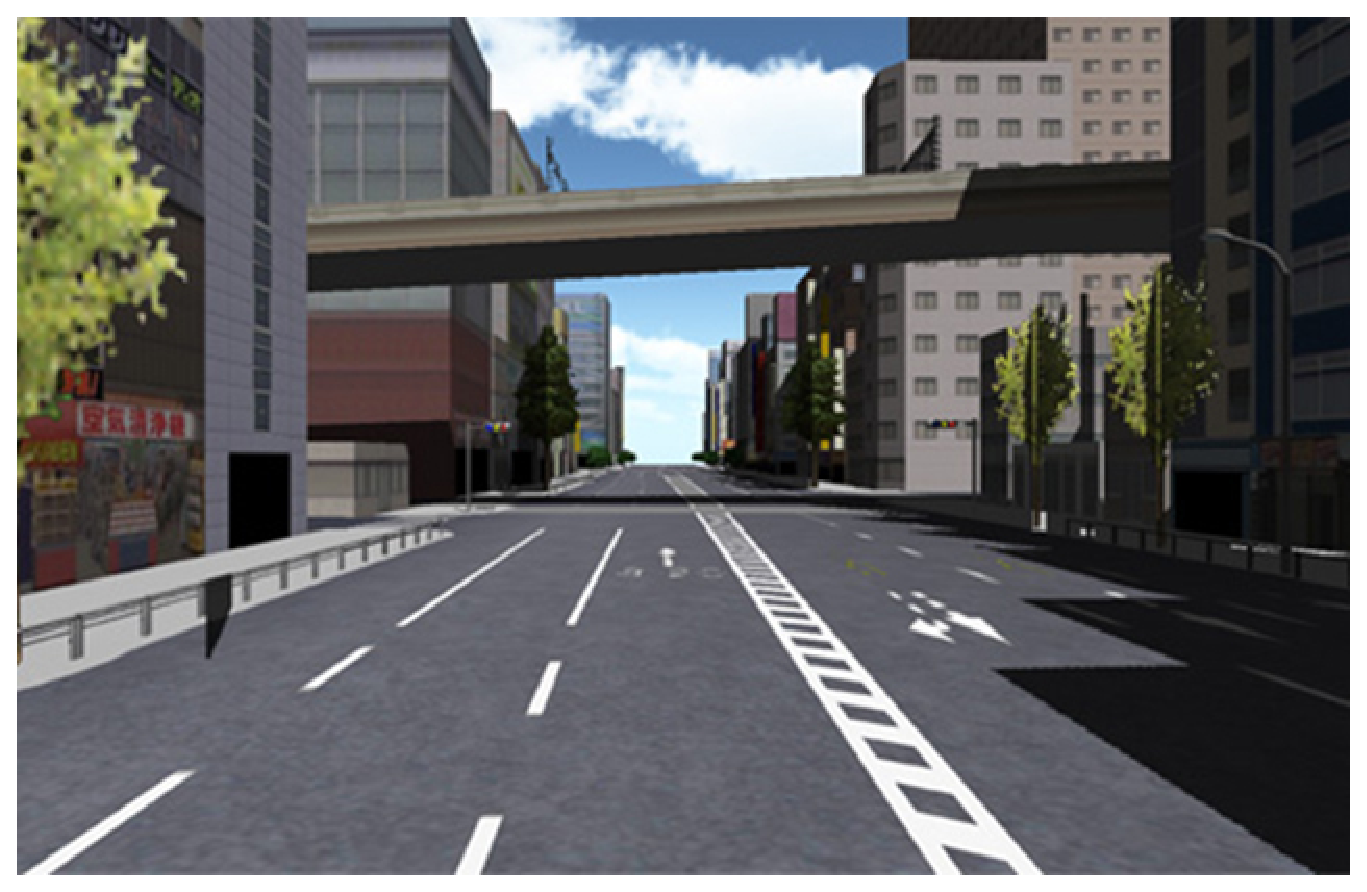
\includegraphics[width=0.8\textwidth]{chap2-figure/akihabara3D.eps}
	\caption{3D都市モデル空間例\protect \footnotemark[1]}
	\label{fig:akihabare}
\end{figure}

\begin{figure}[tbp]
	\centering
			\includegraphics[width=0.8\textwidth]{chap2-figure/ue.eps}
	\caption{3D都市モデル空間上部\protect \footnotemark[1]}
	\label{fig:ue}
\end{figure}

\footnotetext [1]{この作品は『ZENRIN City Asset SeriesTM』を素材として制作されている.}

\section{処理の流れ}
提案システムの処理の流れについて述べる.処理の流れを図\ref{fig:片桐2}に示す.
提案システムの開始方法は,HMDをつなげたPCのマウスを左クリック又はキーボードのスペースキーで開始される.HMDに提示される開始画面を図\ref{fig:start}に示す.開始後,キャラクタの一人称視点の映像が提示され歩行が開始される.開始後の画面を図\ref{fig:gemestart}に示す.患者は設定時間が終了するまで下肢リハビリを続ける.設定した時間が終了すると,図\ref{fig:end}の画面が提示される.
\begin{figure}[tbp]
	\centering
			\includegraphics[width=0.3\textwidth]{chap2-figure/katagiri2.eps}
	\caption{処理の流れ}
	\label{fig:片桐2}
\end{figure}

\begin{figure}[tbp]
	\centering
			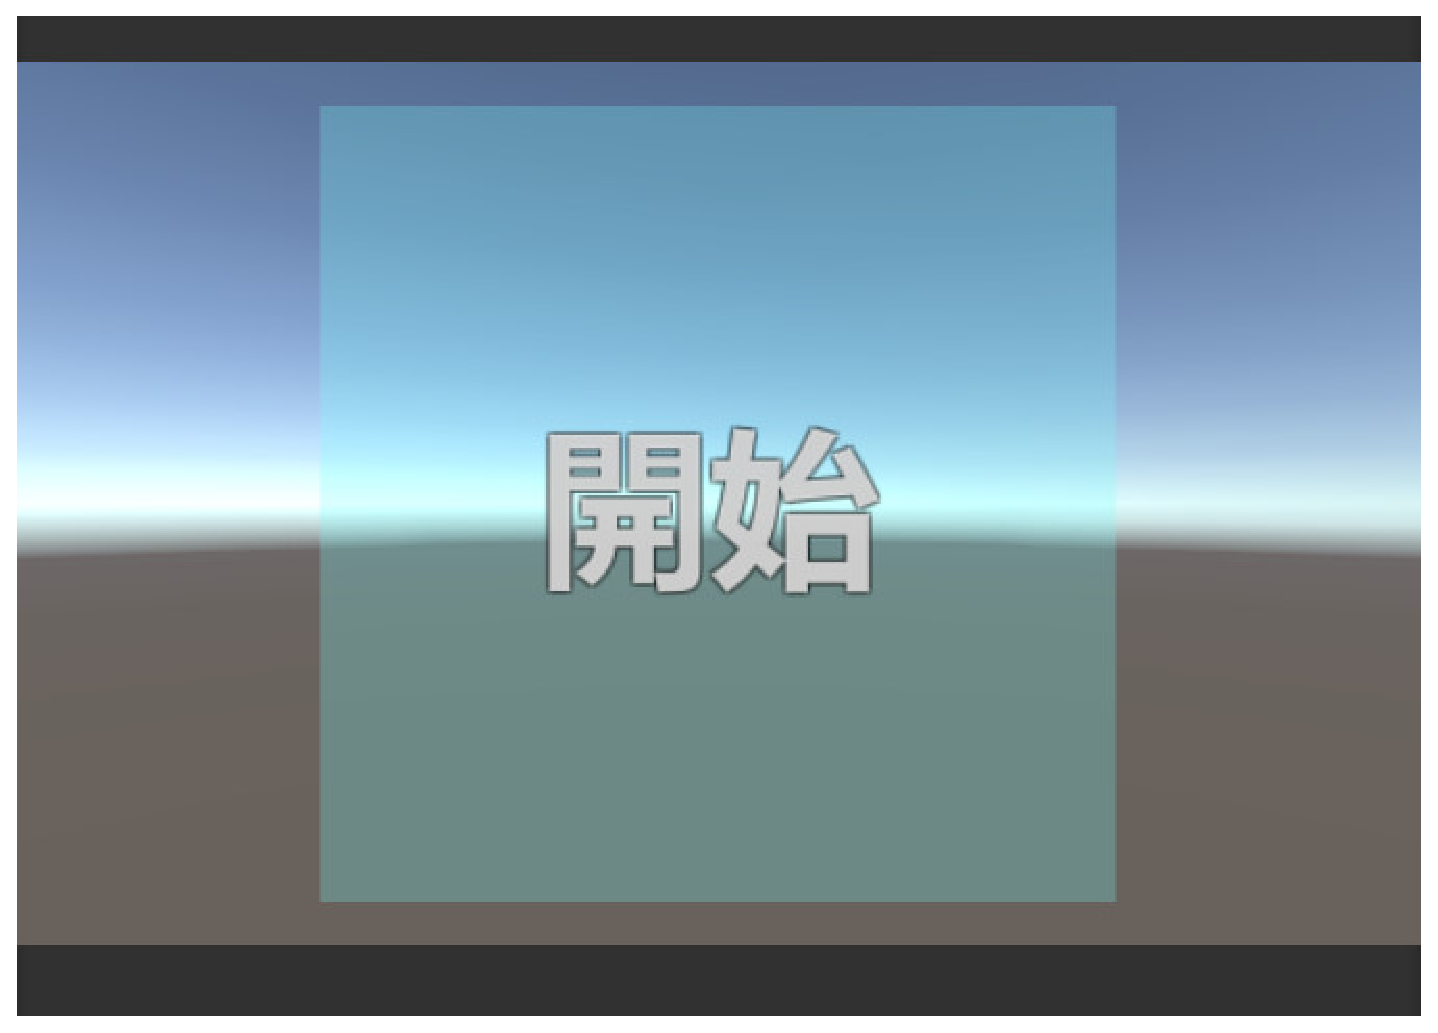
\includegraphics[width=0.9\textwidth]{chap2-figure/start.eps}
	\caption{スタート画面}
	\label{fig:start}
\end{figure}

\begin{figure}[tbp]
	\centering
			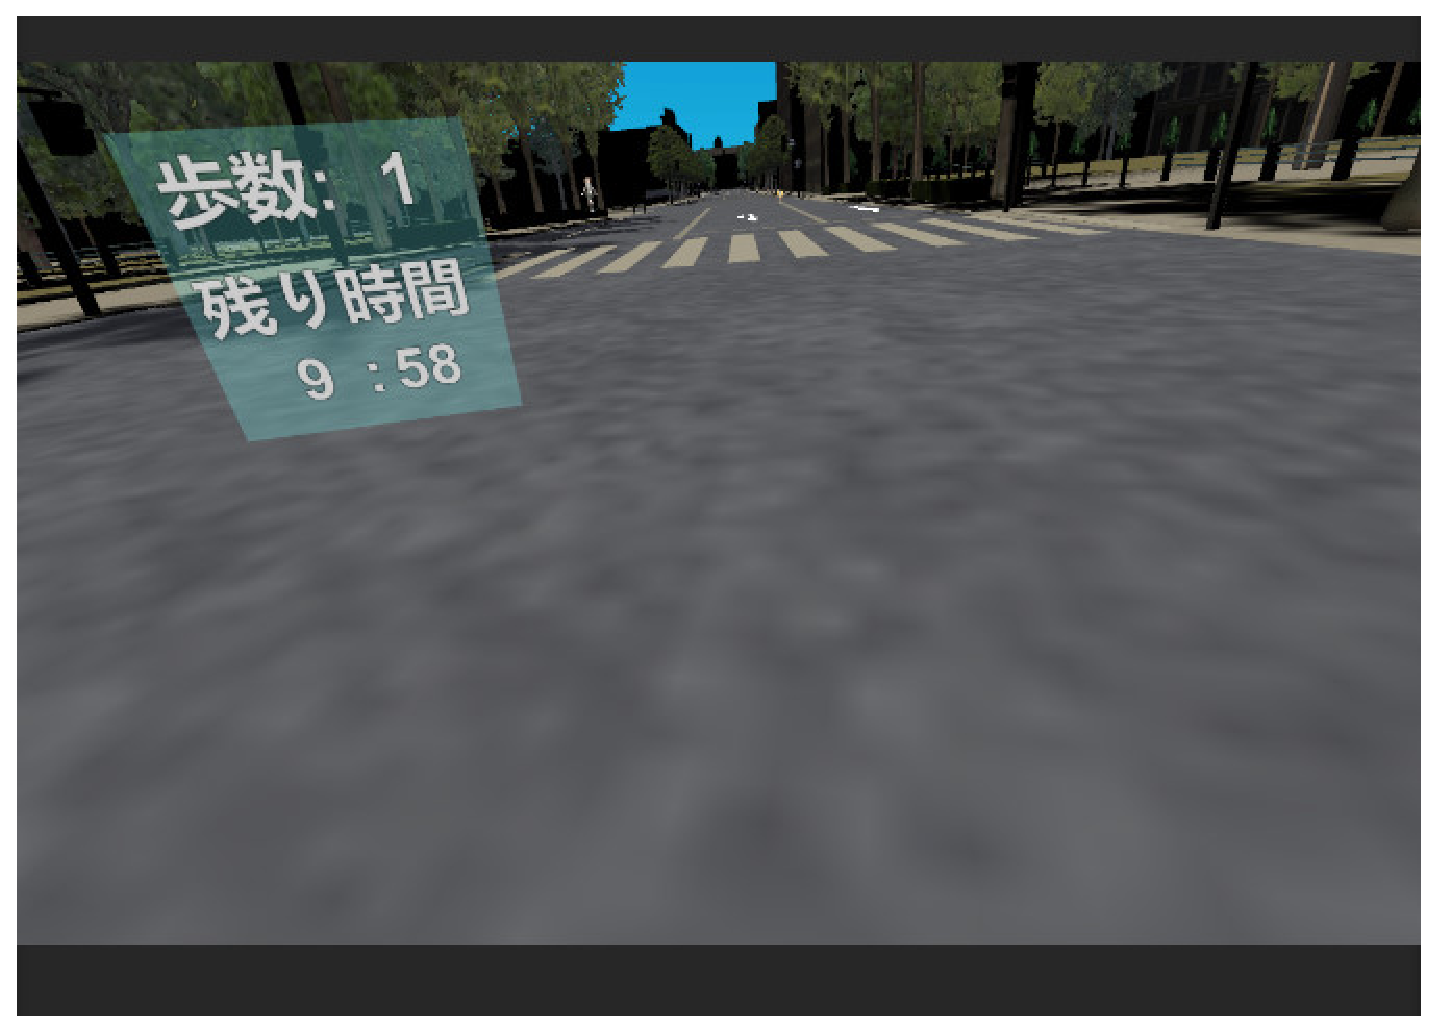
\includegraphics[width=0.9\textwidth]{chap2-figure/midstream-1.eps}
	\caption{開始後画面}
	\label{fig:gemestart}
\end{figure}

\begin{figure}[tbp]
	\centering
			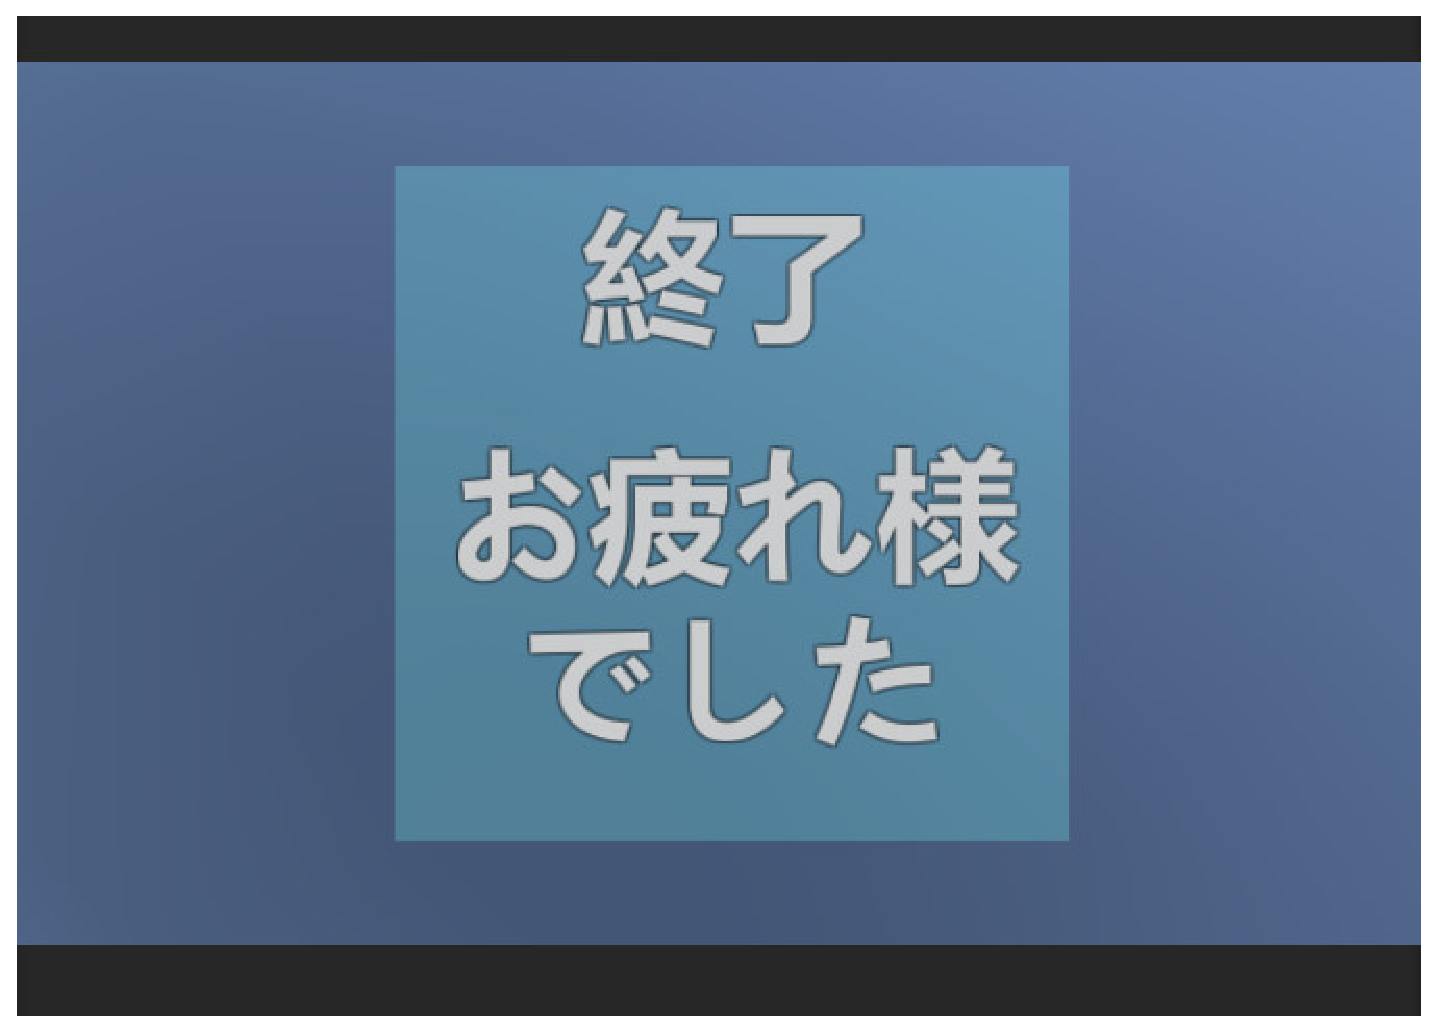
\includegraphics[width=0.9\textwidth]{chap2-figure/end.eps}
	\caption{終了画面}
	\label{fig:end}
\end{figure}

\subsection{歩行距離の設定}
CGキャラクタの歩行距離は,ベッド型の下肢リハビリ装置から読み取れる動作周波数から計算され,動作周波数$N$秒間の1周期ごとに,CGキャラクタが$M$m進む.設定した時間までCGキャラクタは歩行動作を続ける.

\subsection{キャラクタの視点設定}
HMDには,センサが内蔵されており,頭部の動きに応じて映像がリアルタイムに追従するので,仮想空間に没入できる利点がある.すなわち,患者が頭部を動かすと,仮想空間内に配置されたCGキャラクタの視点も追従して変わり,HMDの持つ没入感という利点を活かしている.図\ref{fig:geammidstream}に,プレイ途中に頭部を動かした一例を示す.

\begin{figure}[tbp]
	\centering
			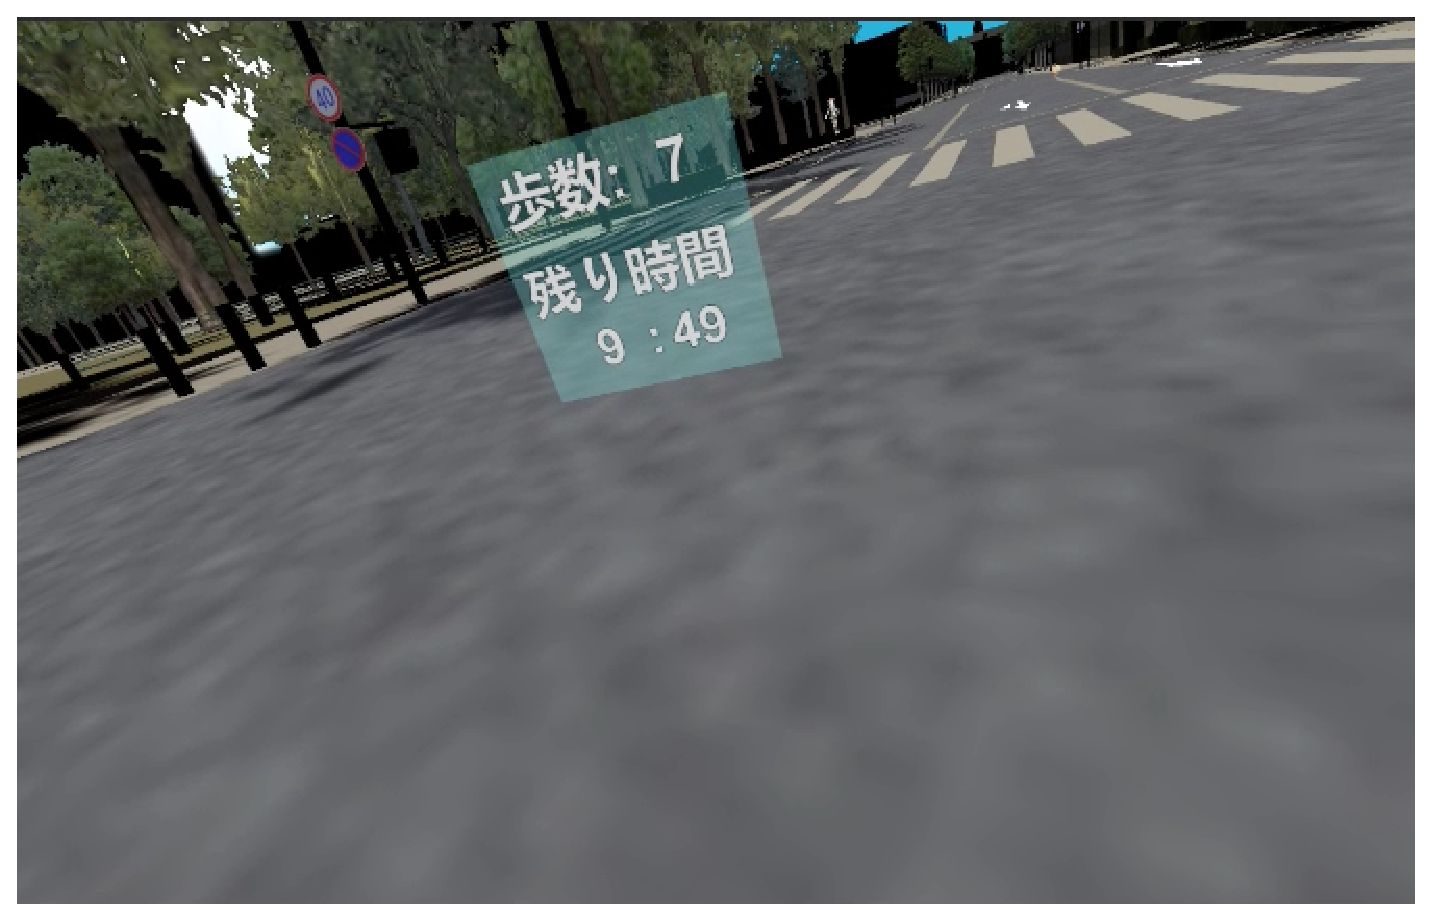
\includegraphics[width=0.9\textwidth]{chap2-figure/midstream-2.eps}
	\caption{プレイ途中視点を変えた図}
	\label{fig:geammidstream}
\end{figure}

\section{むすび}
本章では,ベッド型の下肢リハビリ装置から読み取れる動作周波数から計算されるCGキャラクタの歩行距離によって,3D都市モデル空間でのCGキャラクタの移動を行う手法について述べた.ベッド型の他動歩行器と同時に体験するシステムのためのキャラクタの視点の変更を行う手法を記述した.第3章では,大学生の被験者に対して行った提案システムに関するアンケート評価について述べる.
% Local Variables: 
% mode: japanese-LaTeX
% TeX-master: "root"
% End: 
